\documentclass[12pt,letterpaper, onecolumn]{exam}
\usepackage{amsmath}
\usepackage{amssymb}
\usepackage{graphicx}
\usepackage{setspace}
\usepackage{nicefrac}
\setcounter{MaxMatrixCols}{20}
\usepackage[lmargin=.75in, rmargin=.75in]{geometry}  %For centering solution box
\lhead{Optimal Estimation}
\rhead{Noah Miller}
\thispagestyle{empty}   %For removing header/footer from page 1

\begin{document}

\begingroup
\centering
\LARGE Optimal Estimation\\
\LARGE Homework 3 \\[0.5em]
\large \today\\[0.5em]
\large Noah Miller\par
\large 903949330\par
\large MECH 7710\par
\endgroup
\pointsdroppedatright   %Self-explanatory
\printanswers
\renewcommand{\solution}{\noindent\textbf{Ans:}\enspace}   %Replace "Ans:" with starting keyword in solution box
\vspace{.5cm}

\noindent Note: All problems are to be sampled at 10~Hz ($T_s = 0.1$) except for problem 3.

\noindent Also, all data is available on Canvas.
\begin{questions}
    \question{Kalman Filter at its best -- simulation (actually the Kalman filter is also quite reliable when we have an excellent model and low noise sensors). Suppose we have a second-order system that we are regulating about zero (position and velocity) by wrapping an \textit{optimal} control loop around the system. The new dynamics of the continuous time system are given by the closed-loop A matrix:
        \[
            A_{CL} =
            \begin{bmatrix}
                0  & 1    \\
                -1 & -1.4 \\
            \end{bmatrix}
        \]
        Suppose our measurement is simply position $\left(C = \left[\;1 \quad 0\;\right]\right)$. There is a white noise process disturbance $\left(force, B_w = \left[\;0 \quad 1\;\right]^T\right)$ acting on the controlled system.}
    \begin{parts}
        \part{Simulate the controlled system with the disturbance force $\left(1\sigma = 2\right)$ and a sampled sensor noise $\left(1\sigma = 1\right)$ for 100 seconds at a 10~Hz sample rate.}

        \solution{%
            We can setup the simulation by writing out our continuous model (Equation \ref{eq:1}) and measurement model (Equation \ref{eq:2}) and then evaluating both models over a period of 100 seconds with a sample rate of 1 Hertz.
            \begin{equation}
                \mathbf{\dot{x}} = \mathbf{A}_{CL}\mathbf{x} + \mathbf{B}_ww
                \label{eq:1}
            \end{equation}
            Where $\mathbf{\dot{x}}$ is the change in position and velocity over a sample, $\mathbf{A}_{CL}$ is our closed-loop dynamic model, $\mathbf{x}$ is our current position and velocity, $\mathbf{B}_w$ is input disturbance matrix, and $w$ is our process noise.
            \begin{equation}
                \mathbf{Y} = \mathbf{C}\mathbf{x} + \eta
                \label{eq:2}
            \end{equation}
            Where $\mathbf{Y}$ is our measurement of position, $\mathbf{C}$ is our output matrix, and $\eta$ is our sensor noise.
            \begin{figure}[!h]
                \centering
                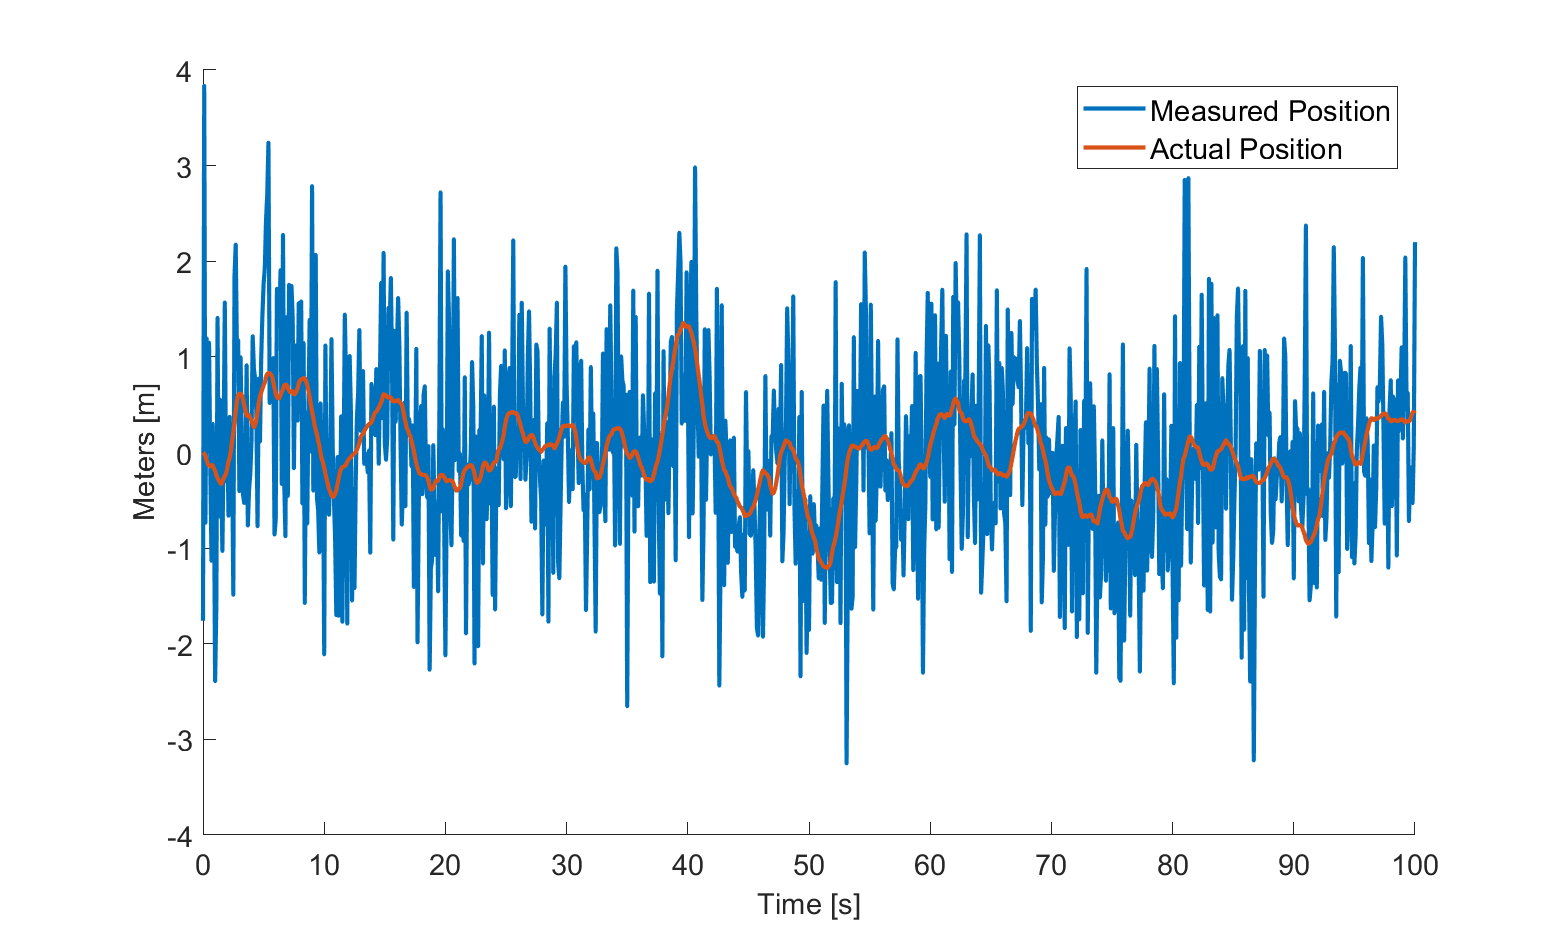
\includegraphics[width=0.85\linewidth]{Q1_simulation.png}
                \caption{Actual and measured position simulated over 100 seconds with a 0.1 second time step.}
                \label{fig:1}
            \end{figure}
        }
        \clearpage
        \part{What is $Q$,$\mathbf{Q}_d$, and $R_d$?}

        \solution{%
        We know $Q$ to be the variance of the process noise, or $E\left[ww^T\right]$. Executing this expectation tells us that \[Q \approx 4. \]
        $\mathbf{Q}_d$ is the discrete process noise and can be evaulated by first finding the discrete dynamic model, $A_d$. We can determine $A_d$ by usings Bryson's trick as seen in Equation \ref{eq:3}.
        \begin{equation}
            \begin{split}
                \mathbf{A}_d & = \left(e^{\mathbf{s}\Delta t}_{2,2}\right)^T\\
                \mathbf{s} & =
                \begin{bmatrix}
                    -\mathbf{A}_{CL} & \left(\mathbf{B}_w Q \mathbf{B}_w\right) \\
                    0                & \mathbf{A}_{CL}^T                        \\
                \end{bmatrix} \\
                & =
                \begin{bmatrix}
                    0 & -1  & 0 & 0    \\
                    1 & 1.4 & 0 & 40   \\
                    0 & 0   & 0 & -1   \\
                    0 & 0   & 1 & -1.4 \\
                \end{bmatrix} \\
                \mathbf{s}\Delta t & =
                \begin{bmatrix}
                    0  & -.1 & 0  & 0    \\
                    .1 & .14 & 0  & 0.4  \\
                    0  & 0   & 0  & -.1  \\
                    0  & 0   & .1 & -.14 \\
                \end{bmatrix} \\
                e^{\mathbf{s}\Delta t} & =
                \begin{bmatrix}
                    0.994 & -0.107 & -0.001 & -0.021 \\
                    0.107 & 1.144  & 0.021  & 0.431  \\
                    0     & 0      & 0.995  & -0.093 \\
                    0     & 0      & 0.093  & 0.864  \\
                \end{bmatrix} \\
                \mathbf{A}_d & =
                \begin{bmatrix}
                    0.995  & 0.093 \\
                    -0.093 & 0.864 \\
                \end{bmatrix}\\
            \end{split}
            \label{eq:3}
        \end{equation}
        From Equation \ref{eq:3} we can calculate the discrete process noise as $\mathbf{Q}_d = \mathbf{A}_de^{\mathbf{s}\Delta t}_{1,2}$.
        \begin{equation}
            \begin{split}
                \mathbf{Q}_d & =
                \begin{bmatrix}
                    0 & 0    \\
                    0 & 0.43 \\
                \end{bmatrix} \\
            \end{split}
            \label{eq:4}
        \end{equation}
        $R_d$ is similar to $Q$ but instead of the process noise, it is the variance of the sensor noise. We can approximate $R_d$ as \[R_d \approx 1. \]
        }
        \part{Calculate the steady state Kalman gain for the system. This can be done in one of many ways: iterate the Kalman filter unit it converges, $dlqe.m$, $dare.m$, $kalman.m$, $dlqr.m$ ($+$ predictor to current estimator trick), etc.
            What is the steady state covariance of the estimates after the time update, $P^{(-)}$, as well as after the measurement update,$P^{(+)}$? Where are the poles of the estimator?}

        \solution{%
        In order to add the Kalman Filter to our existing model, we need to install a time update and measurement update with \textit{a priori} and \textit{a posteriori} covariance estimate to change our Kalman gains as we iterate through time (Equation \ref{eq:5},\ref{eq:6}). Keep in mind, for the following equations, I signify the time update with a superscript $t$ and a measurement update with a superscript $m$. These are typically listed as $-$ and $+$, respectively.
        \begin{equation}
            \begin{split}
                \text{Time} \;&\; \text{Update}\\
                \mathbf{\hat{x}}^t_k & = \mathbf{A}_d \mathbf{\hat{x}}^m_{k-1} \\
                \mathbf{P}^t_k & = \mathbf{A}_d \mathbf{P}^m_k \mathbf{A}_d^T + \mathbf{Q}_k\\
            \end{split}
            \label{eq:5}
        \end{equation}

        \begin{equation}
            \begin{split}
                \text{Measurement} \;&\; \text{Update}\\
                \mathbf{L}_k & = \mathbf{P}^t_k \mathbf{C}^T_d \left(\mathbf{C}_d \mathbf{P}^t_k \mathbf{C}_d^T + R_k\right)^{-1}\\
                \mathbf{P}^m_k & = \left(\mathbf{I} - \mathbf{L}_k \mathbf{C}_d\right)\mathbf{P}^t_k \\
                \mathbf{\hat{x}}^m_k & = \mathbf{\hat{x}}^t_k + \mathbf{L}_k \left(Y_k - \mathbf{C}_d \mathbf{\hat{x}}^t_k\right) \\
            \end{split}
            \label{eq:6}
        \end{equation}
        From Figure \ref{fig:2} we see that the steady state Kalman gains, $\mathbf{L}_{k_{ss}}$, settle to
        $\begin{bmatrix}
                0.196 \\
                0.212 \\
            \end{bmatrix}$.

        \begin{figure}[!h]
            \centering
            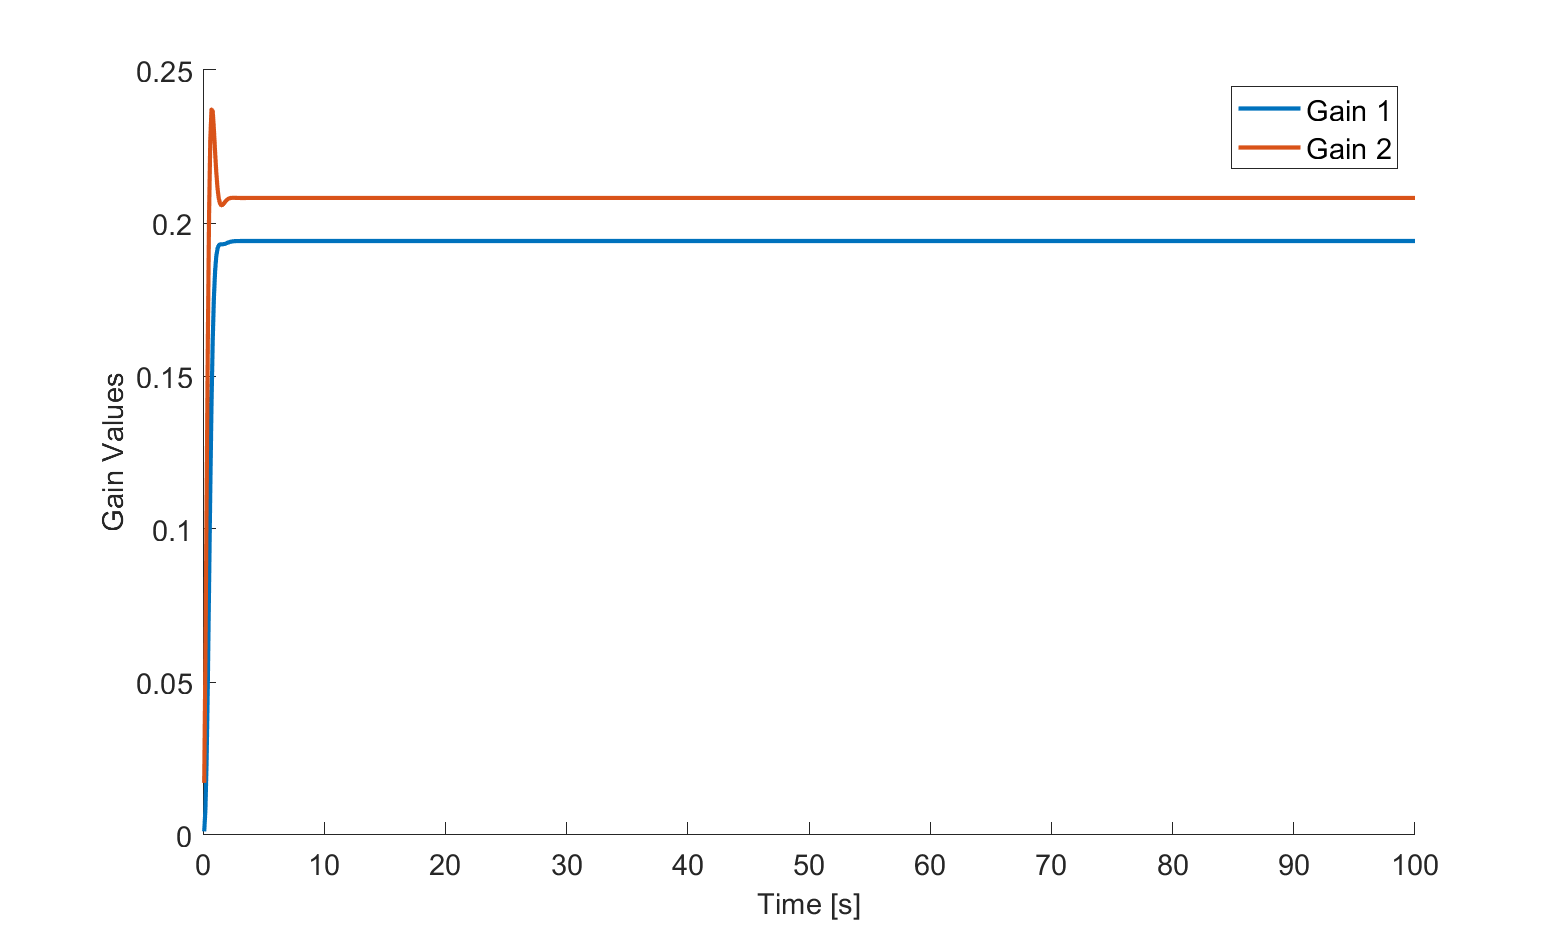
\includegraphics[width=0.60\linewidth]{Q1_gain.png}
            \caption{Values of $\mathbf{L}_k$ as time increases.}
            \label{fig:2}
        \end{figure}

        We also find that steady state \textit{a priori} covariance matrix equals
        \[ \mathbf{P}^t_k =
            \begin{bmatrix}
                0.23857 & 0.2583 \\
                0.2583  & 1.0723 \\
            \end{bmatrix} \]
        and that the steady state \textit{a posteriori} covariance matrix is equal to
        \[ \mathbf{P}^m_k =
            \begin{bmatrix}
                0.19187 & 0.20773 \\
                0.20773 & 1.0175  \\
            \end{bmatrix} \]

        In order to find the poles of the estimator, we can find the eigenvalues of our estimator $\mathbf{A}$ matrix that I will call $\mathbf{A}_o$.
        \begin{equation}
            \begin{split}
                \mathbf{A}_o & = \mathbf{A}_d - \mathbf{L}_{k_{ss}}\mathbf{C}\\
                \mathbf{A}_o & =
                \begin{bmatrix}
                    0.799  & 0.093 \\
                    -0.305 & 0.864 \\
                \end{bmatrix}
            \end{split}
            \label{eq:7}
        \end{equation}
        Then simply using $>>eig$ in MATLAB produces estimator poles of
        \[s_{1,2} = 0.83213 \pm 0.1654i \]
        }
        \clearpage
        \part{Now use the steady state Kalman filter to generate an estimate $\big(\hat{x}\;\text{and}\;\hat{\dot{x}}\big)$ of the 2 states over time. Calculate the norm of the standard deviation of the errors of each state. \[N = \sqrt{\big(std\big(\dot{x} - \hat{\dot{x}}\big)\big)^2 + \left(std\big(x - \hat{x}\big)\right)^2} \]}

        \solution{%
            \begin{figure}[!h]
                \centering
                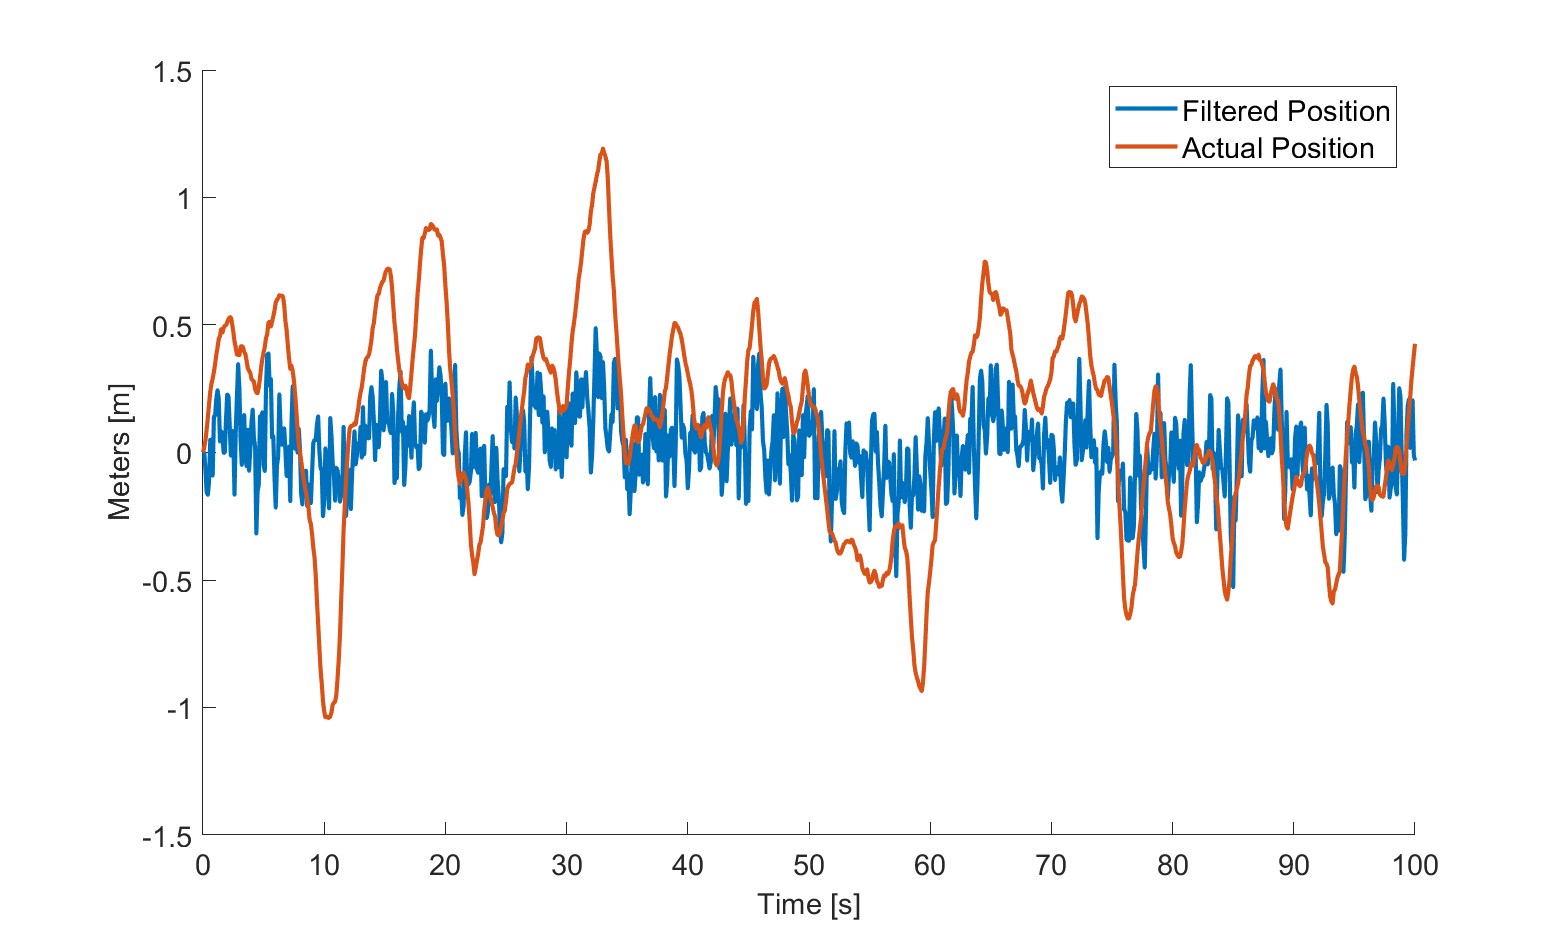
\includegraphics[width=\linewidth]{Q1_filter.png}
                \caption{Filtered Position versus Actual Position}
                \label{fig:3}
            \end{figure}

            Using the equation provided we calculate a value of $N = 0.58579$.
        }
        \part{%
            Change the ratio of the $Q$ and $R$ weights in the Kalman filter design (and repeat part (d) with new Kalman gain but DO NOT regenerate a new $x$ and $\dot{x}$) and determine the effect on the estimation errors. For what ratio of $Q$ and $R_d$ are the errors minimized?

            Note: Often in practice we do not know the actual $Q$ and $R_d$ so these tend to be "tuning" parameters we can use to tune our filter. However, according to Kalman, the estimation errors are only minimized if we use the $Q$ and $R_d$ of the physical system.}

        \solution{%
            Using a multivariable minimization function ($>>fmincon$), I found the lowest normalized standard deviation of our state error to be $~0.49$ with $R_d = 0.95$ and $Q = 0.33$. This gives us a $Q$ to $R_d$ ratio of about $0.38$. The trend seems to be that as one lowers the process noise, $N$ will also decrease. I am not sure if $R_d$ had a profounding affect on $N$.
        }

    \end{parts}
    \clearpage
    \question{Download the data \textit{hw3\_2}} from the website. The data is in the form $\left[\;\mathbf{t} \quad \mathbf{y}\;\right]$. Suppose we want to design an estimator to estimate the bias in the measurement $y$. We believe that the bias, $x$, is constant so we use the model given by
    \[\dot{x} = 0\]
    \[y_k = x_k + \nu_k \]
    \[\nu_k \sim N(0,1) \]
    \begin{parts}
        \part{Run the Kalman filter estimator with $Q_d = 0$. What at happens when $t$ becomes greater than 100 seconds? Why? Calculate the steady state Kalman gain $L_{ss}$. Plot $L(k)$. This is known as the filter "going to sleep" (i.e. becomes a least squares estimator). }

        \part{To offset this problem we will "tune" $Q_d$ to track the bias. What is the effect of changing $Q_d$ on the ability to track the step change in the bias? Try values of $Q_d$ from $0.0001$ to $0.01$ and plot $L(k)$ as well as the estimate of the bias $(\hat{x})$. What is the trade-off?}

        \part{Now filter the measurement using the first-order low-pass filter
            \[H(z)=  \frac{\sqrt{Q_d}}{z - \left(1 - \sqrt{Q_d}\right)} \]
            Use the command:
            \[yf = filter(numd,dend,y,y0)\]}

        \part{How does this compare to the Kalman filter solution? Why are these two filters the same for this problem.}
    \end{parts}
    \clearpage
    \question{Design a “Navigation” type Kalman filter to estimate the states [East, North Radar\_Bias, Psi, Gyro\_Bias]. (Note: this is a non-linear problem that requires an Extended Kalman Filter (EKF) to do correctly.)

        However we can solve the problem in one of two ways:
        \begin{itemize}
            \item[i.] linearize the equations about the nominal operating point and produce a constant A matrix for that operating point
            \item[ii.] simply update the A matrix at every time step with our measurements or estimates
        \end{itemize}
        Download the data \textit{hw3\_3} from the website and run the filter sampled at 5 Hz}
    \begin{parts}
        \part{How did you choose the covariance values for $Q_d$ (especially for the radar and gyro biases)?}

        \part{How does the bias estimation compare to least squares solution? How the bias estimate compare to the Recursive Least Squares solution if you make the covariance ($Q_d$) of the bias estimates equal to zero?}

        \part{Integrate the last 40 seconds of data to see how well you have estimated the biases. This can simply be done by "turning off" the measurements in the observation matrix! Why do the bias estimates remain constant during the 40 second "outage"?}

    \end{parts}
    \clearpage
    \question{Estimator for Vehicle Dynamics. The yaw dynamics of a car (for a stability control system) can be described by the following model (at $25~\frac{m}{s}$):
        \begin{equation*}
            \begin{split}
                \dot{X} & =
                \begin{bmatrix}
                    -2.62 & 12 \\
                    -0.96 & -2 \\
                \end{bmatrix}
                \begin{bmatrix}
                    \dot{\psi} \\
                    \beta      \\
                \end{bmatrix} +
                \begin{bmatrix}
                    14 \\
                    1  \\
                \end{bmatrix}
                \delta\\
                y_k & =
                \begin{bmatrix}
                    1 & 0 \\
                \end{bmatrix}
                X_k + \nu_k\\
            \end{split}
        \end{equation*}
        where:
        \begin{equation*}
            \begin{split}
                \dot{psi} & = \text{Vehicle Yaw Rate}\\
                \beta & = \text{Vehicle Sideslip Angle}\\
                \delta & = \text{Steer Angle}\\
                \nu_k & = \text{Sample Sensor Noise}\\
            \end{split}
        \end{equation*}
    }
    \begin{parts}
        \part{Assuming we can only measure the yaw rate $(\nu_k \sim N[0,(0.1)^2 ])$, design a Kalman filter to do full state estimation (select a reasonable $Q_d$ ). Provide a unit step steer input and estimate both states. On one page plot the actual states and estimated states (use $>>subplot(2,2,n)$ for each of the two states). Where are the steady state poles of the estimator?

            Now, somebody has loaded the trunk of the vehicle with bricks, changing the CG of the vehicle so now the actual model (at $25~\frac{m}{s}$) is:
            \begin{equation*}
                \begin{split}
                    \dot{X} & =
                    \begin{bmatrix}
                        -2.42 & 4  \\
                        -0.99 & -2 \\
                    \end{bmatrix}
                    \begin{bmatrix}
                        \dot{\psi} \\
                        \beta      \\
                    \end{bmatrix} +
                    \begin{bmatrix}
                        18 \\
                        1  \\
                    \end{bmatrix} \delta\\
                    y_k & =
                    \begin{bmatrix}
                        1 & 0 \\
                    \end{bmatrix}
                    X_k + \nu_k\\
                \end{split}
            \end{equation*}
            Note: We do not know that somebody has loaded the trunk and that the CG has changed, therefore we must use the model of part (a) in our Kalman filter.
        }

        \part{Redo part (a). Can you estimate the slip angle correctly? Try various $Q_d$.}

        \part{Now lets say we have a noisy measurement of the slip angle ($\eta_k \sim N\left[0,0.5^2\right]$):
            \[
                y_k =
                \begin{bmatrix}
                    1 & 0 \\
                    0 & 1 \\
                \end{bmatrix} X_k +
                \begin{bmatrix}
                    \nu_k  \\
                    \eta_k \\
                \end{bmatrix}
            \]
            Assuming the sensor noises are uncorrelated, what is $R$?}

        \part{Redo part (a). What is the effect of changing the element of $Q_d$ associated with the slip angle estimate. What must $Q_d$ equal to ensure an unbiased estimate of the states (How much filtering does that provide)?}

    \end{parts}
    \clearpage
    \question{(\textbf{OPTIONAL}) Estimator of a non-minimum phase system. Consider the system dynamics
        \begin{equation*}
            \begin{split}
                \dot{x_1} & = w\\
                \dot{x_2} & = -x_1 - 2x_2 + w\\
            \end{split}
        \end{equation*}
        with continuous measurements $y(t) = x_2(t) + v(t)$. The measurements and process noise are both independent white noise processes (spectral densities $R_v$ and $R_w$ respectively).
    }
    \begin{parts}
        \part{Find the transfer function $G_{yw}(s)$ from $w(s)$ to $y(s)$ and identify the poles and zeros. Recall that right-half place zeros are called non-minimum phase.}

        \part{Use this transfer function to sketch the symmetric root locus for the time-invariant estimator poles vs. $\frac{R_w}{R_v}$. Clearly demonstrate that one of the estimator poles tends towards $s  = -1\;\text{as}\;\frac{R_v}{R_w} \rightarrow 0$, even though there is no zero there (only a reflected one). Confirm that this implies that part of the estimation error will attenuate faster than $e^-t$ even with noise-free measurements.}

        \part{Use the solution of the steady-state Riccati equation to show that as $\frac{R_v}{R_w} \rightarrow 0$, the
            \begin{equation*}
                P \rightarrow
                \begin{bmatrix}
                    2R_w            & -\sqrt{R_w R_v} \\
                    -\sqrt{R_w R_v} & \sqrt{R_w R_v}  \\
                \end{bmatrix}
            \end{equation*}}

        \part{Use this results to confirm that $x_1$ can not be estimated perfectly, even with
            $R_v \rightarrow 0$.}

        \part{Comment on the impact of the non-minimum phase zero on our ability to estimate this system's state.}
    \end{parts}
\end{questions}

\end{document}